\documentclass[12pt]{article}
\usepackage[final]{graphicx}
\usepackage{minted}
\usepackage{multicol}
\usepackage{subcaption}
\usepackage[english]{babel}

\title{Transformer polarity test}
\author{}
\date{}

\begin{document}
\vspace*{\fill}
\begin{center}

    \emph{Heaven's Light is Our Guide} \\
    \textbf{Rajshahi Universiy of Engineering and Technology} \\

    \begin{figure}[h]
        \centering
        
\includegraphics[scale=.34]{images/RUET_logo.png}
        \label{fig:ruet_logo}
    \end{figure}
    \vspace{5mm}

    \textbf{Course Code}\\
    ECE 2208\\
    \vspace{3mm}
    \textbf{Course Title}\\
    Electrical Machines - I Sessional

    \vspace{5mm}
    \textbf{Experiment Date:} {October 4, 2023,}\\
    \textbf{Submission Date:} {October 18, 2023}\\

    \vspace{5mm}
    \textbf{Lab Report 1:} Polarity test of a transformer.\\

    \vspace{15mm}

    \begin{tabular}{c|c}
        \textbf{Submitted to} & \textbf{Submitted by} \\
        Md. Omaer Faruq Goni  & Md. Tajim An Noor     \\
        Lecturer              & Roll: 2010025         \\
        Dept of ECE, RUET     &                       \\
    \end{tabular}

\end{center}
\vspace*{\fill}

\pagebreak

\tableofcontents

\maketitle
\section{Introduction}

Electricity flows from a point with higher voltage to one with lower voltage due to the difference in potential. This concept is related to electrical polarity, which denotes the direction of current flow. In direct current (DC) systems, one terminal is consistently positive, while the other is negative, indicating a unidirectional current flow. In alternating current (AC) systems, the polarity of the terminals changes periodically, causing the current direction to also change accordingly.\cite{polarity}\\

To identify the voltage polarity in the mutual inductance of two windings, we employ the dot convention. There are two commonly used principles:
\begin{itemize}
    \item When current enters the dotted terminal of one winding, the voltage induced in the other winding will be positive at the dotted terminal of the second winding.
    \item If current exits the dotted terminal of one winding, the induced voltage in the other winding will be negative at the dotted terminal of the second winding.
\end{itemize}

\subsection{Polarity Test}
We can categorize the polarity of the transformer to two types:
\begin{itemize}
    \item Additive Polarity
    \item Subtractive Polarity
\end{itemize}

\subsubsection*{Additive Polarity}
In additive polarity, the voltage $(V_c)$ between the primary side $(V_a)$ and the secondary side $(V\_b)$ will be the sum of both high voltage and the low voltage, i.e. we will get\\ \indent $V_c = V_a + V_b$

\subsubsection*{Subtractive Polarity}
In subtractive polarity, the voltage $(V_c)$ between the primary side $(V_a)$ and the secondary side $(V_b)$ will be the difference of both high voltage and the low voltage, i.e. we will get\\ \indent $V_c = V_a - V_b$\\
In subtractive polarity, if $(V_c = V_a - V_b)$, it is a step-down transformer and if $(V_c = V_b - V_a)$, it is a step-up transformer.\cite{polarity}


\subsection{Circuit Diagrams}
\begin{figure}[H]
    \begin{subfigure}{\textwidth}
        \centering
        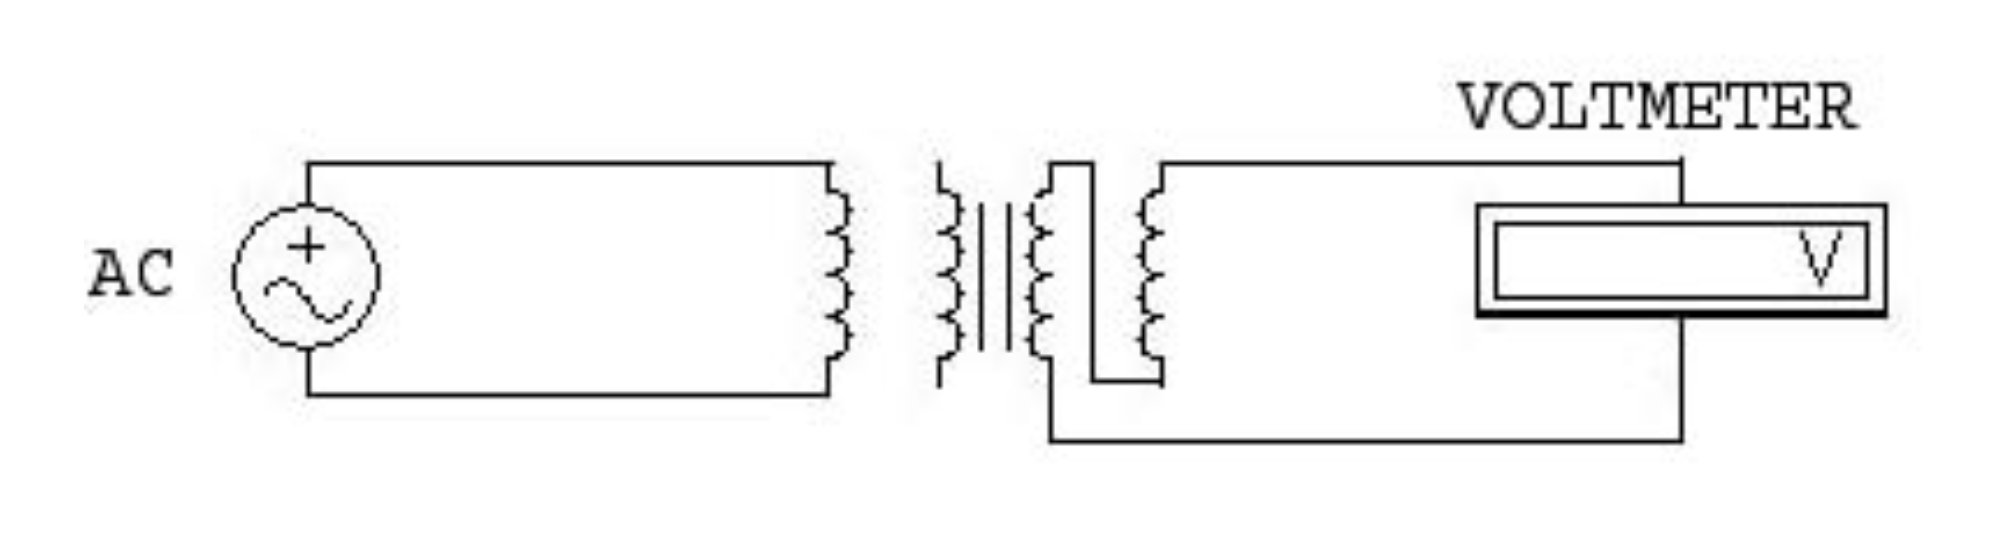
\includegraphics[width=.8\linewidth]{images/output/add.png}
        \caption{Additive (step-up) polarity.}
        \label{fig:sfig1}
    \end{subfigure}
    \begin{subfigure}{\textwidth}
        \centering
        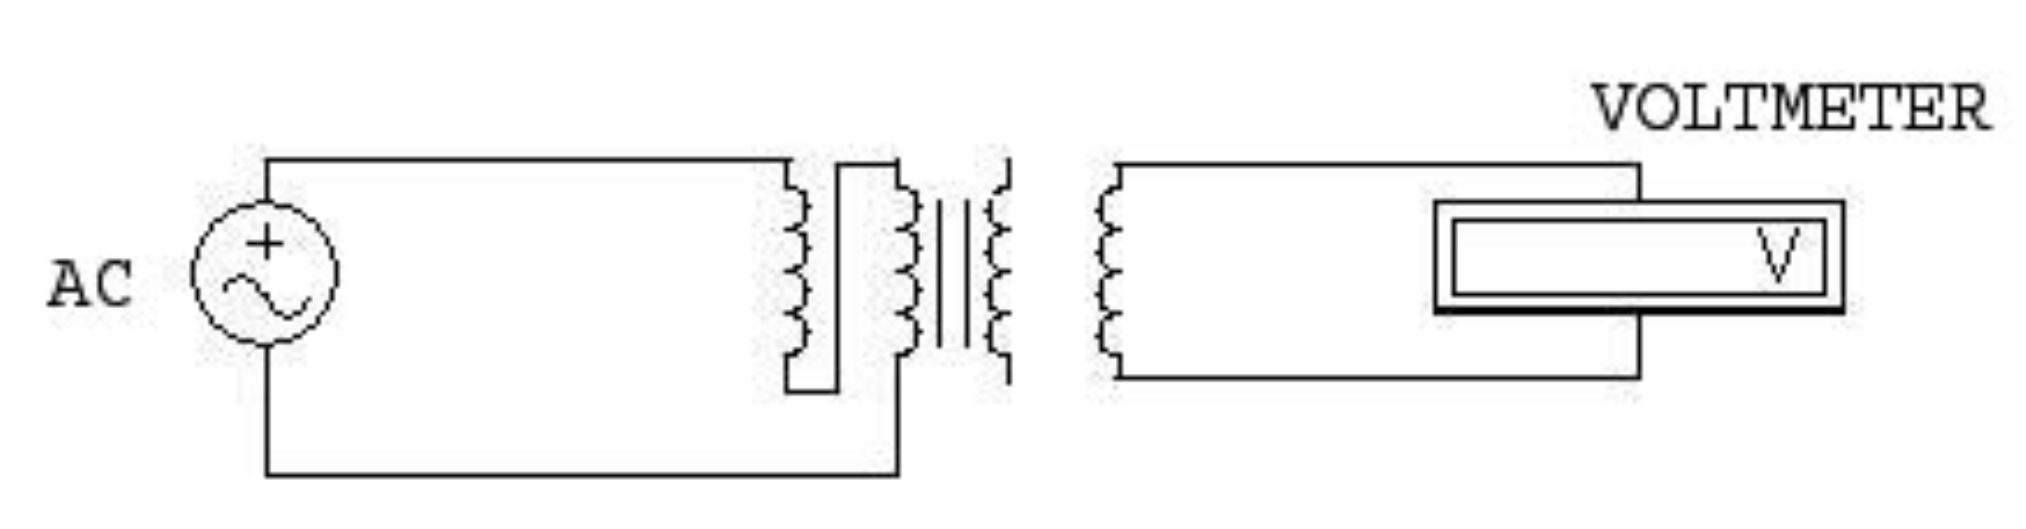
\includegraphics[width=.8\linewidth]{images/output/sub.png}
        \caption{Subtractive (step-down) polarity.}
        \label{fig:sfig2}
    \end{subfigure}
    \caption{Circuit diagrams for polarity test of transformer windings.}
    \label{fig:fig}
\end{figure}
\pagebreak
\section{Tools Used}
\begin{itemize}
    \item Transformer (150V - 1A)
    \item Connecting wires
    \item Multimeter
    \item AC (220V)
    \item Variac (0-250V)
\end{itemize}

\section{Data}
\subsection*{Step Up: Connected in additive polarity}
Primary coil is the 1\textsuperscript{st} coil, all others are considered secondary.
\begin{table}[H]
    \centering
    \begin{tabular}{|c|l|c|c|}
        \hline
        Input Voltage & Connected Windings (Secondary) & Output Voltage (V) & $N_p/N_s$ \\
        \hline
        50            & 1                              & 50                 & 1         \\
        \hline
        50            & 1, 2                           & 100                & 1/2       \\
        \hline
        50            & 1, 2, 3                        & 150                & 1/3       \\
        \hline
        50            & 1, 2, 3, 4                     & 200                & 1/4       \\
        \hline
    \end{tabular}
    \caption{Step up}
\end{table}

\subsection*{Step Down: Connected in subtractive polarity}
Secondary coil is the 4\textsuperscript{th} coil, all others are considered primary.
\begin{table}[H]
    \centering
    \begin{tabular}{|c|l|c|c|}
        \hline
        Input Voltage & Connected Windings (Primary) & Output Voltage (V) & $N_p/N_s$ \\
        \hline
        100           & 1, 2, 3, 4                   & 25                 & 1/4       \\
        \hline
        100           & 1, 2, 3                      & 33.33              & 1/3       \\
        \hline
        100           & 1, 2                         & 50                 & 1/2       \\
        \hline
        100           & 1                            & 100                & 1         \\
        \hline
    \end{tabular}
    \caption{Step down}
\end{table}

\pagebreak
\section{Discussion}
In this experiment, to check the polarity of the windings of the transformer used, we connect the windings in series one by one and see if the voltage is increased of not. Of the four windings in the transformer, the one where the AC voltage was connected, is the primary coil. All the others are secondary coils. \\
Now, for the step-up operations, we first connected the 1st \& 2nd winding, these two will now act as the secondary winding. Upon measuring, we check if the output or secondary coils voltage is twice the input voltage (as the windings are of same number of turns, $V_p/V_s = 1$, so with 2 coils, $V_s/V_p = 2$). If it wasn't doubled, the connections were reversed and the additive polarity was found. \\
In this way, the other two windings were added in series and checked if the secondary voltage was four times the input voltage $(V_s/V_4 = 4)$.\\
Now for subtractive polarity, One by one, the connections were reversed to make the transformer step-down.


\section{Conclusion}
When the additive polarity is checked, the windings all together created a step-up transformer. Ass in additive connection, the total number of winding turns was more in the secondary side than the primary side. And in subtractive polarity, the winding became less than the primary side in the secondary side thus making it step down. \\
Utmost caution was exercised in this experiment as it was done with AC voltage supply. The connections were given carefully with caution as not to touch any open terminals.

\bibliographystyle{IEEEtran}
\bibliography{ref}

\end{document}